\documentclass{article}
\usepackage{tikz}
\usetikzlibrary{arrows.meta, positioning}

\begin{document}

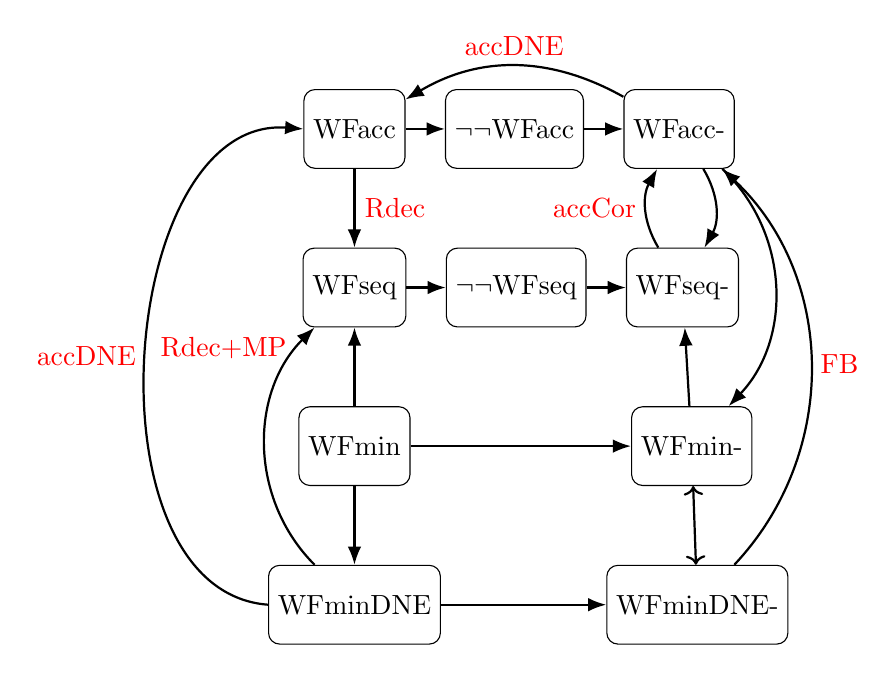
\begin{tikzpicture}[
  node distance=1cm and .5cm,
  box/.style={draw, rectangle, rounded corners, minimum width=1cm, minimum height=1cm, align=center},
  arrow/.style={-{Latex}, thick}
]

% Row 1: WFacc
\node[box] (WFacc) {WFacc};
\node[box, right=of WFacc] (NNWFacc) {$\lnot\lnot$WFacc};
\node[box, right=of NNWFacc] (WFaccM) {WFacc-};

\draw[arrow] (WFacc) -- (NNWFacc);
\draw[arrow] (NNWFacc) -- (WFaccM);
\draw[arrow, bend right] (WFaccM) to node[above, text=red] {accDNE} (WFacc);

% Row 2: WFind
% \node[box, below=of WFacc] (WFind) {WFind};
% \node[box, right=of WFind] (NNWFind) {$\lnot\lnot$WFind};
% \node[box, right=of NNWFind] (WFindM) {WFind-};

% \draw[arrow] (WFind) -- (NNWFind);
% \draw[arrow] (NNWFind) -- (WFindM);

% Row 3: WFseq
\node[box, below=of WFacc] (WFseq) {WFseq};
\node[box, right=of WFseq] (NNWFseq) {$\lnot\lnot$WFseq};
\node[box, right=of NNWFseq] (WFseqM) {WFseq-};

\draw[arrow] (WFseq) -- (NNWFseq);
\draw[arrow] (NNWFseq) -- (WFseqM);

% Row 4: WFmin -> WFmin-
\node[box, below=of WFseq] (WFmin) {WFmin};
\node[box, right=2.8cm of WFmin] (WFminM) {WFmin-};

\draw[arrow] (WFmin) -- (WFminM);

% Row 5: WFminDNE -> WFminDNE-
\node[box, below=of WFmin] (WFminDNE) {WFminDNE};
\node[box, right=2.1cm of WFminDNE] (WFminDNEM) {WFminDNE-};

\draw[arrow] (WFminDNE) -- (WFminDNEM);

% Arrows between rows
% \draw[arrow, <->] (WFacc) -- (WFind);
% \draw[arrow, <->] (NNWFacc) -- (NNWFind);
% \draw[arrow, <->] (WFaccM) -- (WFindM);

\draw[arrow] (WFacc) to node[right, text = red] {Rdec} (WFseq);
\draw[arrow, bend left] (WFaccM) to (WFseqM);
\draw[arrow, bend left] (WFseqM) to node[left, text=red] {accCor} (WFaccM);  
\draw[arrow, bend left = 45] (WFaccM) to (WFminM);  


\draw[arrow] (WFmin) -- (WFseq);
\draw[arrow] (WFminM) -- (WFseqM);
\draw[arrow] (WFmin) -- (WFminDNE);
\draw[arrow, <->] (WFminM) -- (WFminDNEM);

\draw[arrow, bend left=90] (WFminDNE) to node[left, text = red] {accDNE} (WFacc);
\draw[arrow, bend left=45] (WFminDNE) to node[pos=0.9, left, text=red] {Rdec$+$MP} (WFseq);
\draw[arrow, bend right=45] (WFminDNEM) to node[right, text=red] {FB} (WFaccM);


\end{tikzpicture}

\end{document}
